% This is samplepaper.tex, a sample chapter demonstrating the
% LLNCS macro package for Springer Computer Science proceedings;
% Version 2.20 of 2017/10/04
%
\documentclass[runningheads, envcountsame, a4paper]{llncs}
%

\usepackage{graphicx}
% Used for displaying a sample figure. If possible, figure files should
% be included in EPS format.
%
\usepackage{hyperref}
%\usepackage[colorlinks]{hyperref}
% If you use the hyperref package, please uncomment the following line
% to display URLs in blue roman font according to Springer's eBook style:
\renewcommand\UrlFont{\color{blue}\rmfamily}


\usepackage{alltt}
%\usepackage{pslatex}
%\usepackage{epigraph}
%\usepackage{verbatim}
\usepackage{latexsym}
\usepackage{array}
\usepackage{comment}
%\usepackage{makeidx}
%\usepackage{indentfirst}
%\usepackage{verbatim}
%\usepackage{color}
%\usepackage{url}
%\usepackage{xspace}
%\usepackage{hyperref}
%\usepackage{stmaryrd}
\usepackage{amsmath}
\usepackage{amssymb}  % mathcal
%\usepackage{graphicx}
%\usepackage{euscript}
\usepackage{mathtools}
%\usepackage{mathrsfs}
%\usepackage{multirow,bigdelim}
%\usepackage{subcaption}
%\usepackage{placeins}
\usepackage{csvsimple}
\usepackage{array}

%\usepackage{geometry}
%\geometry{
%     top=25pt, bottom=14pt, inner=21pt, outer=21pt,
%     paperwidth=5.5in, paperheight=8.5in,
%     }
\usepackage{color}



%% Some recommended packages.
\usepackage{booktabs}   %% For formal tables:
                        %% http://ctan.org/pkg/booktabs
\usepackage{subcaption} %% For complex figures with subfigures/subcaptions
                        %% http://ctan.org/pkg/subcaption
\captionsetup{compatibility=false}

\usepackage{multirow}

\usepackage{placeins}

\usepackage{lmodern}

\usepackage{listings}
\lstdefinelanguage{ocanren}{
keywords={run, conde, fresh, let, in, match, with, when, class, type,
object, method, of, rec, repeat, until, while, not, do, done, as, val, inherit,
new, module, sig, deriving, datatype, struct, if, then, else, open, private, virtual, include, success, failure, switch, 
true, false},
sensitive=true,
commentstyle=\small\itshape\ttfamily,
keywordstyle=\ttfamily\textbf,
identifierstyle=\ttfamily,
basewidth={0.5em,0.5em},
columns=fixed,
mathescape=true,
fontadjust=true,
literate={fun}{{$\lambda$}}1 {->}{{$\to$}}3 {===}{{$\equiv$}}1 {=/=}{{$\not\equiv$}}1 {|>}{{$\triangleright$}}3 {\\/}{{$\vee$}}2 {/\\}{{$\wedge$}}2 {^}{{$\uparrow$}}1 
%{[]}{{\texttt|[]|}}1
,
morecomment=[s]{(*}{*)}
}

\lstset{
%mathescape=true,
%basicstyle=\small,
%identifierstyle=\ttfamily,
%keywordstyle=\bfseries,
%commentstyle=\scriptsize\rmfamily,
%basewidth={0.5em,0.5em},
%fontadjust=true,
language=ocanren
}

\newcommand{\lstquot}[1]{``\lstinline{#1}''}
\newcommand{\sembr}[1]{\llbracket{#1}\rrbracket}
\newcommand\false{$f\!alse$}
\newcommand\myif{i\!f}


\def\transarrow{\xrightarrow}
\newcommand{\setarrow}[1]{\def\transarrow{#1}}

\def\padding{\phantom{X}}
\newcommand{\setpadding}[1]{\def\padding{#1}} 

\def\subarrow{}
\newcommand{\setsubarrow}[1]{\def\subarrow{#1}}

\newcommand{\trule}[2]{\dfrac{#1}{#2}}
\newcommand{\crule}[3]{\dfrac{#1}{#2},\;{#3}}
\newcommand{\withenv}[2]{{#1}\vdash{#2}}
\newcommand{\trans}[3]{{#1}\transarrow{\padding{\textstyle #2}\padding}\subarrow{#3}}
\newcommand{\ctrans}[4]{{#1}\transarrow{\padding#2\padding}\subarrow{#3},\;{#4}}
\newcommand{\llang}[1]{\mbox{\lstinline[mathescape]|#1|}}
\newcommand{\pair}[2]{\inbr{{#1}\mid{#2}}}
\newcommand{\inbr}[1]{\left<{#1}\right>}
\newcommand{\highlight}[1]{\color{red}{#1}}
%\newcommand{\ruleno}[1]{\eqno[\scriptsize\textsc{#1}]}
\newcommand{\ruleno}[1]{\mbox{[\textsc{#1}]}}
\newcommand{\rulename}[1]{\textsc{#1}}
\newcommand{\inmath}[1]{\mbox{$#1$}}
\newcommand{\lfp}[1]{fix_{#1}}
\newcommand{\gfp}[1]{Fix_{#1}}
\newcommand{\vsep}{\vspace{-2mm}}
\newcommand{\supp}[1]{\scriptsize{#1}}
\renewcommand{\sembr}[1]{\llbracket{#1}\rrbracket}
\newcommand{\cd}[1]{\texttt{#1}}
\newcommand{\free}[1]{\boxed{#1}}
\newcommand{\binds}{\;\mapsto\;}
\newcommand{\dbi}[1]{\mbox{\bf{#1}}}
\newcommand{\sv}[1]{\mbox{\textbf{#1}}}
\newcommand{\bnd}[2]{{#1}\mkern-9mu\binds\mkern-9mu{#2}}
\newcommand{\meta}[1]{{\mathcal{#1}}}
\newcommand{\dom}[1]{\mathtt{dom}\;{#1}}
%\newcommand{\primi}[2]{\mathbf{#1}\;{#2}}
\renewcommand{\dom}[1]{\mathcal{D}om\,({#1})}
\newcommand{\ran}[1]{\mathcal{VR}an\,({#1})}
\newcommand{\fv}[1]{\mathcal{FV}\,({#1})}
\newcommand{\tr}[1]{\mathcal{T}r_{#1}}
\newcommand{\diseq}{\not\equiv}
\newcommand{\reprfunset}{\mathcal{R}}
\newcommand{\reprfun}{\mathfrak{f}}
\newcommand{\cstore}{\Omega}
\newcommand{\cstoreinit}{\cstore_\epsilon^{init}}
\newcommand{\csadd}[3]{add(#1, #2 \diseq #3)}  %{#1 + [#2 \diseq #3]}
\newcommand{\csupdate}[2]{update(#1, #2)}  %{#1 \cdot #2}
\newcommand{\primi}[1]{\mathbf{#1}}
\newcommand{\sem}[1]{\llbracket #1 \rrbracket}
\newcommand{\ir}{\ensuremath{\mathcal{S}}}
\usepackage{tikz}
\newcommand*\circled[1]{\tikz[baseline=(char.base)]{
    \node[shape=circle,draw,inner sep=1pt] (char) {#1};}}

\renewcommand{\le}{\ensuremath{\leqslant}}

\let\emptyset\varnothing
\let\eps\varepsilon

\newtheorem{Observation}{Observation}

\usepackage{float}

%\usepackage{hyperref}
%\usepackage[colorlinks]{hyperref}
\hbadness=99999  % suppress warnings about underfullness

\begin{document}
%
\title{Relational Synthesis for Pattern Matching\thanks{The reported study was funded by RFBR, projects number 18-01-00380 and 19-31-90053.}}

%\thanks{This work was partially supported by the grant 18-01-00380 from The Russian Foundation for Basic Research.\\
%
%\titlerunning{Abbreviated paper title}
% If the paper title is too long for the running head, you can set
% an abbreviated paper title here
%
\author{
%Anonymous author(s)
  Dmitry Kosarev\inst{1,2,3}\orcidID{0000-0002-6773-5322} \and
Petr Lozov\inst{1,2,4}\orcidID{0000-0003-3563-2828}\and
Dmitry Boulytchev\inst{1,2,5}\orcidID{0000-0001-8363-7143}
}
%
\authorrunning{D. Kosarev et al.}
% First names are abbreviated in the running head.
% If there are more than two authors, 'et al.' is used.
%
\institute{Saint Petersburg State University, Russia \and
JetBrains Research, Russia\and 
\email{Dmitrii.Kosarev@pm.me}  \and 
\email{lozov.peter@gmail.com} \and 
\email{dboulytchev@math.spbu.ru}
}
%\institute{Anonymous institute}
%
\maketitle              % typeset the header of the contribution
\setcounter{footnote}{0}

%
\begin{abstract}
   We apply relational programming techniques to the problem of synthesizing efficient implementation for a pattern matching construct. Although in principle
   pattern matching can be implemented in a trivial way, the result suffers from inefficiency in terms of both performance and code size. Thus, in implementing functional languages alternative, more elaborate  approaches are widely used. However, as there are multiple kinds and flavors of pattern
   matching constructs, these approaches have to be specifically developed and justified for each concrete inhabitant of the pattern matching ``zoo.'' We formulate the
   pattern matching synthesis problem in relational terms and develop optimizations which improve the efficiency of the synthesis and guarantee the
   optimality of the result. Our approach is based on relational representations of both the high-level semantics of pattern matching and the semantics of
   an intermediate-level implementation language. This choice make our approach, in principle, more scalable as we only need to modify the high-level semantics in order
   to synthesize the implementation of a new feature. Our evaluation on a set of small samples, partially taken from existing literature shows, that our framework is
   capable of synthesizing optimal implementations quickly. Our in-depth stress evaluation on a number of artificial benchmarks, however,
   has shown the need for future improvements.
\keywords{relational programming \and relational interpreters \and pattern matching.}

\end{abstract}

\section{Introduction}

Relational programming is an approach, based on the idea of describing programs not as functions, but 
as relations, without distinguishing between the arguments and the result value. This technique makes it 
possible to ``query'' programs in various ways, for example, to execute them ``backwards'', finding
all sets of arguments for a given result. Relational behavior can be reproduced using a number of
logic programming languages, such as Prolog, Mercury~\cite{Mercury}, 
or Curry~\cite{Curry}. 
There is also a family of embedded DSLs, specifically designed for writing declarative relational
programs that originates from \miniKanren~\cite{TRS}. \miniKanren is a minimalistic 
declarative language, initially developed for Scheme/Racket. The smallest implementation of \miniKanren 
is reported to comprise of only 40 LOC~\cite{MicroKanren,2016}; there are also more elaborate versions, including
\miniKanren with constraints~\cite{CKanren,CKanren1}, user-assisted search~\cite{Guided}, nominal unification~\cite{AlphaKanren},
etc. Due to its simplicity, \miniKanren was implemented for more than 50 other languages, such as
Haskell, Go, Smalltalk, and OCaml. In a nutshell, miniKanren introduces a minimalistic set of constructs to describe
relations over a set of syntactic terms, thus providing the same expressivity as a pure core of conventional
logic programming\footnote{A detailed miniKanren to Prolog comparison can be found at \url{http://minikanren.org/minikanren-and-prolog.html}}. 

\miniKanren has proven to be a useful tool to provide elegant solutions for various problems, otherwise considered as
non-trivial~\cite{WillThesis}. One of the most promising areas of application for \miniKanren is the implementation of
\emph{relational interpreters}. Such interpreters are capable not only to interpret programs in various directions, but also
to infer programs on the basis of expected input-output specification~\cite{Untagged}.

Being quite simple and easy to use by design, in implementation \miniKanren introduces some subtleties. Under the hood, \miniKanren 
uses a complete interleaving search~\cite{Search}. This search is guaranteed to find all existing solutions; however, it can diverge, when no 
solution exists. In reality, this amounts to divergence in a number of important cases~--- for example, when a program is asked to 
return \emph{all} existing solutions, or when the number of requested solutions exceeds the number of existing ones.
It is often possible to refactor the specification of a concrete query to avoid the divergence, but this has to be done for every execution
``direction'' of interest that compromises the idea of fully declarative relational programming.

The specifications that do not diverge even when no solutions exist, are called \emph{refutationally complete}~\cite{WillThesis}. Writing 
refutationally complete relational specifications nowadays requires knowledge of \miniKanren implementation intrinsics, and is not always
possible due to the undecidability of the fundamental computability problems. However, by developing a more advanced search it is possible
to make more specifications refutationally complete.

In this work we address one particular problem that often leads to refutational incompleteness~--- the non-commutativity of
conjunction. We present an optimization technique that is based on a certain non-termination test. Our optimization
is \emph{online} (performed during the search), \emph{non-intrusive} (does not introduce new constructs and does not require
any changes to be made to the existing specifications), and \emph{conservative} (applied only when the divergence
is detected). We prove that for the queries that return a finite number of answers, our optimization preserves convergence. 
We also demonstrate the application of the optimization for a number of interesting and important problems.

We express our gratitude to William Byrd and the reviwers of this paper for their constructive remarks and suggestions.


\section{Related works}
\label{sec:related}

Although semantics of pattern matching can be given as a sequence of srutinee's sub expression comparisons (Figure~\ref{fig:matchpatts}) effective compilers don't follow this approach. One can either optimise runtime cost by minimizing amount of checks performed or static cost by minimizing the size of generated code. \emph{Decision trees} are good for the first criteria, because they check every subexpression not more than once. \emph{Backtracking automata} are rather compact but in some cases can perform repeated checks.


Minimizing the size of decision tree is  NP-hard (\cite{macqueen1985}, without proof) and usually various heuristics are applied during compilation, for example: count of nodes, length of the longest path, average length of all paths. The paper~\cite{Ramsey2000} performs experimental evaluation of these heuristics.

The matching compilers for strict languages can work in \emph{direct} or \emph{indirect} styles. The first ones return effective code immediately. In the second style to construct final answer some post processing is required. It can vary from easy simplifications to complicated supercompilation techniques~\cite{Setsoft1996}. The main drawback of indirect style is that size of intermediate data structures can be exponentially large.

For strict languages it is allowed to check sub expressions in any order. For lazy languages pattern matching should evaluate only these sub expressions which are necessary for performing pattern matching, if not careful pattern matching can change termination behavior of the program.  In general lazy languages setup more constraints on pattern matching and because of that allow lesser set of heuristics.

A few approaches for checking sub expressions in lazy langauges has been proposed~\cite{Augustsson1985,Laville1991}. \cite{laville1991} models values in lazy languages using \emph{partial terms}, although this approach doesn't scale to types with infinite constructor sets (like integers). In  the \cite{suarez1993} the similar approach is extended by special treatment of overlapping patterns. Pattern matching has been compiled to decision trees~\cite{maranget1992} and later \cite{maranget1992} into \emph{decision DAGs} that allow in some cases to make code smaller.

TODO: mention 3 papers about strict languages.

\section{The Pattern Matching Synthesis Problem}

We describe here a simplified view on pattern matching which does not incorporate some practically important aspects of the construct such as
name bindings in patterns, guards or even semantic actions in branches. In a purified form, however, it  represents the essence of pattern
matching as an ``inspect-and-branch'' procedure. Other features can be easily added later once a solution for the essential part of the problem
is found.

First, we introduce a finite set of \emph{constructors} $\mathcal C$, equipped with arities, a set of values $\mathcal{V}$
and a set of patterns $\mathcal{P}$:
 
\[
 \begin{array}{rcll}
    \mathcal{C} & = & \{ C_1^{k_1}, \dots, C_n^{k_n} \}\\
    \mathcal{V} & = & \mathcal{C}\,\mathcal{V}^*\\  
    \mathcal{P} & = & \_ \mid \mathcal{C}\,\mathcal{P}^*
 \end{array}
\]

We define a matching of a value $v$ (\emph{scrutinee}) against an ordered non-empty sequence of patterns $p_1,\dots,p_k$ by means of the following
relation

\[
\setarrow{\xrightarrow}
\trans{\inbr{v;\,p_1,\dots,p_k}}{}{i},\,1\le i\le k+1
\]

\noindent which gives us the index of the leftmost matched pattern or $k+1$ if no such pattern exists. We use an auxiliary relation $\inbr{;}\subseteq\mathcal{V}\times\mathcal{P}$
to specify the notion of a value matched by an individual pattern (see Fig.~\ref{fig:match1pat}). The rule \ruleno{Wildcard} says that
a wildcard pattern ``\_'' matches any value, and \ruleno{Constructor} specifies that a constructor pattern matches exactly those values which
have the same constructor at the top level and all subvalues matched by corresponding subpatterns. The definition of ``$\xrightarrow{}{\!\!}$'' is
shown on Fig.~\ref{fig:matchpatts}. An auxiliary relation
 ``$\xrightarrow{}{}_{\!\!*}$'' 
is introduced to specify the left-to-right matching strategy, and we
use current index as an environment. An important rule, $\ruleno{MatchOtherwise}$ specifies that if we exhausted all the patterns with no matching we stop with
the current index (which in this case is equal to the number of patterns plus one).

\begin{figure}[t]
   \renewcommand*{\arraystretch}{2}
   \[
   \begin{array}{cr}
     \inbr{v;\,\_} & \ruleno{Wildcard} \\
     \trule{\forall i\;\inbr{v_i;\,p_i}}{\inbr{C^k\,v_1\dots v_k;\,C^k\,p_1\dots p_k}},\,k\ge 0 & \ruleno{Constructor}
   \end{array}
   \]
   \caption{Matching against a single pattern}
   \label{fig:match1pat}
\end{figure}

\begin{figure}[t]
   \renewcommand*{\arraystretch}{3}
   \setarrow{\xrightarrow}
   \setsubarrow{_*}
   \[
   \begin{array}{cr}
     \trule{\inbr{v;\,p_1}}
           {\withenv{i}{\trans{\inbr{v;\,p_1,\dots,p_k}}{}{i}}} & \ruleno{MatchHead}\\
     \trule{\neg\inbr{v;\,p_1}\qquad\withenv{i+1}{\trans{\inbr{v;\,p_2,\dots,p_k}}{}{j}}}
           {\withenv{i}{\trans{\inbr{v;\,p_1,\dots,p_k}}{}{j}}} & \ruleno{MatchTail}\\
     \withenv{i}{\trans{\inbr{v;\,\varepsilon}}{}{i}} & \ruleno{MatchOtherwise}\\
     \trule{\withenv{1}{\trans{\inbr{v;\,p_1,\dots,p_k}}{}{i}}}
           {\setsubarrow{}\trans{\inbr{v;\,p_1,\dots,p_k}}{}{i}} & \ruleno{Match}
   \end{array}
   \]
   \caption{Matching against an ordered sequence of patterns}
   \label{fig:matchpatts}
\end{figure}

The relation ``$\xrightarrow{}{}\!\!$'' gives us a \emph{declarative} semantics of pattern matching. Since we are interested in
synthesizing implementations, we need a \emph{programmatical} view on the same problem. Thus, we introduce a language $\mathcal S$
(the ``switch'' language) of test-and-branch constructs:

\[
\begin{array}{rccl}
  \mathcal M & = &       & \bullet \\
             &   & \mid  & \mathcal M\,[\mathbb{N}] \\
  \ir        & = &       & \primi{return}\,\mathbb{N} \\
             &   & \mid  & \primi{switch}\;\mathcal{M}\;\primi{with}\; [\mathcal{C}\; \primi{\rightarrow}\; \ir]^*\;\primi{otherwise}\;\ir
\end{array}
\]
 
Here $\mathcal{M}$ stands for a \emph{matching expression}, which is either a reference to a scrutinee ``$\bullet$'' or
a (multiply) indexed subexpression of a scrutinee. Programs in the switch language can discriminate on the
structure of matching expressions, testing their top-level constructors and eventually returning natural numbers as results.
The switch language is similar to the intermediate representations for pattern matching code used in 
previous works on pattern matching implementation~\cite{maranget2001,maranget2008}, and switch programs are analogous to
\emph{decision trees}.

The semantics of the switch language is given by mean of relations ``$\xrightarrow{}{}_{\!\!\!\mathcal M}$'' and ``$\xrightarrow{}{}_{\!\!\mathcal S}$''
(see Fig.~\ref{fig:matchexpr} and \ref{fig:test-and-branch}). The first one describes the semantics of matching expression, while
the second describes the semantics of the switch language itself. In both cases the scrutinee $v$ is used as an environment ($v\vdash$).


\begin{figure}[t]
  \renewcommand*{\arraystretch}{2}
  \setarrow{\xrightarrow}
  \setsubarrow{_{\mathcal M}}
  \[
  \begin{array}{cr}
    \withenv{v}{\trans{\bullet}{}{v}} & \ruleno{Scrutinee} \\
    \trule{\withenv{v}{\trans{m}{}{C^k v_1\dots v_k}}}{\withenv{v}{\trans{m[i]}{}{v_i}}} & \ruleno{SubMatch} 
  \end{array}
  \]
  \caption{Semantics of matching expression}
  \label{fig:matchexpr}
\end{figure}

\begin{figure}[t]
  \setarrow{\xrightarrow}
  \setsubarrow{_{\mathcal S}}
  \[
  \begin{array}{cr}
    \withenv{v}{\trans{\primi{return}\;i}{}{i}} & \ruleno{Return}\\[10mm]
    
    \trule{\renewcommand*{\arraystretch}{1}
           \begin{array}{c}        
              {\setsubarrow{_{\mathcal M}}\withenv{v}{\trans{m}{}{C^k\ v_1 \dots v_k}}} \\
              \withenv{v}{\trans{s}{}{i}}
           \end{array}
          }    
          {\withenv{v}{\trans{\primi{switch}\;m\;\primi{with}\;[C^k\to s]s^*\;\primi{otherwise}\;s^\prime}{}{i}}} & \ruleno{SwitchMatched}\\[10mm]
          
    \trule{\renewcommand*{\arraystretch}{1}
           \begin{array}{c}        
             {\setsubarrow{_{\mathcal M}}\withenv{v}{\trans{m}{}{D^n\  v_1 \dots v_n}}}\\
             C^k\ne D^n\\
             \withenv{v}{\trans{\primi{switch}\;m\;\primi{with}\;s^*\;\primi{otherwise}\;s^\prime}{}{i}}
           \end{array}
          }
          {\withenv{v}{\trans{\primi{switch}\;m\;\primi{with}\;[C^k\to s]s^*\;\primi{otherwise}\;s^\prime}{}{i}}} & \ruleno{SwitchNotMatched}\\[10mm]
          
    \trule{\withenv{v}{\trans{s}{}{i}}}{\withenv{v}{\trans{\primi{switch}\;m\;\primi{with}\;\varepsilon\;\primi{otherwise}\;s}{}{i}}} & \ruleno{SwitchOtherwise}
  \end{array}
  \]
  \caption{Semantics of switch programs}
  \label{fig:test-and-branch}
\end{figure}

The following observations can be easily proven by structural induction.

\begin{Observation}
  For arbitrary pattern the set of matching values is non-empty:

  \[
  \forall p\in\mathcal P : \{v\in\mathcal V\mid \inbr{v;\,p}\}\ne\emptyset
  \]
\end{Observation}

\begin{Observation}
  Relations ``$\xrightarrow{}{}\!\!\!$'' and ``$\xrightarrow{}{}_{\!\!\mathcal S}$'' are functional and deterministic respectively:

  \[
  \setarrow{\xrightarrow}
  \begin{array}{rcl}
    \forall p_1,\dots,p_k\in\mathcal P,\,\forall v\in \mathcal V,\,\forall \pi\in\mathcal S & : & |\{i\in\mathbb N\mid \trans{\inbr{v;\,p_1,\dots,p_k}}{}{i}\}|=1 \\
                                                                 &  & {\setsubarrow{_{\mathcal S}}|\{i\in\mathbb N\mid \withenv{v}{\trans{\pi}{}{i}}\}|\le 1}
  \end{array}
  \]
\end{Observation}

With these definitions, we can formulate the \emph{pattern matching synthesis problem} as follows: for a given ordered sequence of patterns $p_1,\dots,p_k$ find
a switch program $\pi$, such that

\[
\setarrow{\xrightarrow}
\forall v\in \mathcal V,\; \forall 1\le i\le n+1 : \trans{\inbr{v;\,p_1,\dots,p_n}}{}{i}\Longleftrightarrow{\setsubarrow{_{\mathcal S}}\withenv{v}{\trans{\pi}{}{i}}}\eqno{(\star)}
\]

In other words, program $\pi$ delivers a correct and complete implementation for pattern matching.

\section{Pattern Matching Synthesis, Relationally}

Our idea of using relational programming for pattern matching synthesis is based on the following observations:

\begin{itemize}
\item For the switch language we can implement a relational interpreter $eval^o_\ir$ with the following property: for
  arbitrary $v\in\mathcal V$, $\pi\in\ir$ and $i\in\mathbb N$
 
  \[
  \setarrow{\xRightarrow}
  \setsubarrow{_\ir}
   eval^o_\ir\, v\, \pi\, i \Leftrightarrow \withenv{v}{\trans{\pi}{}{i}}
  \]

  In other words, $eval^o_\ir$ interprets a program $\pi$ for a scrutinee $v$ and returns exactly the same branch (if any)
  which is prescribed by the semantics of the switch language. 
  
\item On the other hand, we can directly encode the declarative semantics of pattern matching as a relational
  program $match^o$ such that for arbitrary $v\in\mathcal V$, $p_i\in\mathcal P$ and $i\in\mathbb N$

  \[
  \setarrow{\xRightarrow}
  match^o\,v\,p_1,\dots,p_k\,i \Leftrightarrow \trans{\inbr{v;\,p_1,\dots,p_k}}{}{i}
  \]

  Again, $match^o$ succeeds with $1\le i\le k$ iff $p_i$ is the leftmost pattern, matching $v$; otherwise it
  succeeds with $i=k+1$.
\end{itemize}

Being relational, both $eval^o_\ir$ and $match^o$ do not just succeed or fail for ground arguments, but also can be \emph{queried} for
arguments with free logical variables, thus performing a search for all substitutions for these variables which make the
relation to hold. This observation leads us to the idea of utilizing the definition of pattern matching
synthesis problem, replacing ``$\xRightarrow{}{}$'' with $match^o$, ``$\xRightarrow{}{}_{\mathcal S}$`` with $eval^o$,
and $\pi$ with a free logical variable $\circled{?}$, which gives us the goal

\[
\forall v\in \mathcal V,\; \forall 1\le i\le n+1 : match^o\,v\,p_1,\dots,p_n\,i\Leftrightarrow eval^o\,v\,\circled{?}\,i
\]

This goal is, however, problematic from relational point of view due to a number of reasons.

First, \textsc{miniKanren} provides rather a limited support for universal quantification. Apart from being inefficient from
performance standpoint, existing implementations either do not support disequality constaints~\cite{eigen}
or quantified qoals with infinite number of answers~\cite{moiseenko}. As we will see below, both restrictions are
violated in our case. Second, there is no direct support for the equivalence of goals (``$\Leftrightarrow$''). Thus,
reducing the original synthesis problem to a viable relational goal involves some ``massaging''.

We eliminate the universal quantification over the infinite set of scrutinees, replacing it by a \emph{finite}
conjunctions over the \emph{complete set of examples}. For a sequence of patterns $p^*$ the
complete set of examples is a finite set of values $\mathcal{E}(p^*)\subseteq\mathcal{V}$ with the following
property:

\[
\forall i\in\mathbb{N},\,(\forall v\in\mathcal{E}(p^*) : \trans{\inbr{v;\,p^*}}{}{i} \Leftrightarrow \forall w\in\mathcal{V}:\trans{\inbr{w;\,p^*}}{}{i})
\]


In particular, for a \emph{concrete} sequence of patterns $p_1,\dots,p_k$, $i\in\mathbb N$ and $v\in\mathcal V$
a goal

\[
  eval^o_\ir\,v\,\circled{?}\,i \wedge match^o\,v\,p_1,\dots,p_k\,i
\]

specifies a search procedure for all switch programs ``$\circled{?}$'' which, being evaluated for $v$, give exactly the same result
as matching against $p_1,\dots,p_k$ (here we denoted by ``$\circled{?}$'' a free logical variable).

 
However, in our concrete
 case there is a simple way to alleviate this problem. Indeed, we may replace universal quantification over $i$ by
 a finite conjunction, as the length of $ps$ is known at the synthesis time. As for the quantification over $s$, for
 any concrete $ps$ we may precompute a \emph{complete set of examples} $\mathcal{E}(ps)\subseteq\mathcal{V}$ with the following
 property:
 
 \[
 \forall i\in\mathbb{N},\,(\forall s\in\mathcal{E}(ps),\,match\, (s, ps, i) \Leftrightarrow \forall s\in\mathcal{V},\,match\, (s, ps, i))
 \]
 
 It easy to see, that for arbitrary $ps$ there exists a finite complete set of examples (indeed, any pattern describes the ``shape''
 of a scrutinee up to some finite depth, beyond which all scrutinees become indistinguishable). Thus, for a given $ps$ we may
 completely eliminate the quantification, reformulating the synthesis problem as
 
 \[
 \bigwedge_{i\in[1\dots|ps|]}\,\bigwedge_{s\in\mathcal{E}(ps)} (eval^o_{\ir}\, (s, p, i) \wedge match\, (s, ps, i))
 \]
 
 We implemented the synthesis framework using \textsc{OCanren}~--- an embedding of \textsc{miniKanren} into \textsc{OCaml}~\cite{ocanren},~---
 and evaluated it on the set of benchmarks, reported in the previous works on \emph{ad-hoc} algorithms for pattern matching
 code generation~\cite{maranget2001,maranget2008}. In comparison with a simplified setting, presented above, our implementation
 deals with a more elaborate pattern matching problem~--- in particular, we support \emph{guard expressions}, name bindings in
 patterns and incorporate a deterministic top-down matching strategy, which is common in functional languages.
 
 Initially, our synthesis did not demonstrate good results. However, we applied the following techniques to improve both the performance
 and the quality of synthesized programs:
 
 \begin{itemize}
 \item we restricted the shape of scrutinees using type information;
 \item we utilized tabling to memoize repeating search steps;
 \item we implemented a pruning technique, which makes the search stop exploring a certain branch if the program, synthesized so far,
   contains too much nesting constructs (this factor can be precomputed by patterns analysis).
 \end{itemize}
 
 With these adjustments, our synthesis framework in a negligible time provides the same results as those reported in the previous works.
 Our future steps include extending the pattern matching language to completely match that of \textsc{OCaml} (for
 now we do not support GADTs), integrate the synthesis into the existing \textsc{OCaml} compiler and evaluate it on a
 set of real-world programs. Another direction is extending the pattern matching language to incorporate features which
 are known to be hard, tedious or error-prone to implement (for example, non-linear patterns).
 

\section{Optimization}
\label{sec:optimization}

In this section we address two aspects of our solution: a number of optimizations which make the search more efficient, and
the way it ends up with the optimal solution.

Relational goal in its final form, presented in the previous section, does not demonstrate a good performance. Thus, we apply a number
of techniques, some of which require extending the implementation of the search. Namely, we apply the following optimizations:

\begin{itemize}
\item We make use of type information to restrict the subset of constructors which may appear in a certain branch of
  program being synthesized.
\item We implement \emph{structural constraints} which allow to restrict the shape of terms during the search, and
  utilize them to implement pruning.  
\end{itemize}

In our formalization we do not make any use of types since as a rule type information does not affect matching. In addition,
utilizing the properties of a concrete type system would make our approach too coupled with this particular type system, hampering
its reusability for other languages. Nevertheless we may use a certain abstraction of type system which would deliver only
that part of information which is essential for our approach to function. Currently, we calculate a type of any matching expression in
program being generated and from this type extract the subset of constuctors which can appear when branching on this expression
is performed. 

\section{Evaluation}
\label{sec:eval}

В данном разделе мы рассмотрим семантику с предикатом, основанном на структурной рекурсии. Также мы представим результаты апробации семантики с тремя разными предикатам на наборе примеров. Для апробации семантика была реализована на языке \textsc{Haskell} в виде интерпретатора. 


% Имперически подобранный критерий
В качестве предиката нам необходим критерий, отличающий вызов, который выгодно раскрутить сейчас от вызова, который стоит отложить. Мы предлагаем predicate by well-quasi-ordering, который эффективен для структурно-рекурсивных отношений. У таких отношений есть хотя бы один аргумент, который структурно убывает с каждым шагом рекурсии. Перестаёт убывать такой аргумент, только когда свободные переменные, которые он содержит, начинают уточняться. И когда все структурные агументы перестанут убывать, мы будем останавливать развёртку вызова.

Сначала определим отношение на кортежах термов.

\begin{definition}
Пусть $t_1^1, \ldots, t_n^1, \, t_1^2, \ldots, t_n^2 \in \mathcal{T}_{\mathcal A}$. Если для любого $i$ верно, что $height(t_i^1) \leq height(t_i^2)$, и существует $j$, для которого $height(t_i^1) < height(t_i^2)$, тогда 
\[
  (t_1^1, \ldots, t_n^1) \leq_h (t_1^2, \ldots t_n^2).
\]
\end{definition}

Отношение ``$\leq_h$'' сравнивает термы по их высоте. Оно требует, чтобы хотя бы один терм левого кордежа был строго короче, чем соответствующий терм из правого кортежа. Остальные левые термы должны быть не длиннее соотвествующих термов в правом кортеже.

\begin{lemma}
\label{lemma:wqo1}
Отношение ``$\leq_h$'' является well-quasi-ordering.
\end{lemma}
Доказывается индукцией по сумме высот всех термов.

Теперь определим отношение на парах из подстановки и реляционного применения.

\begin{definition}
Пусть $\theta_1, \theta_2$ --- подстановки,  $r_1, r_2$ --- реляционные применения. Если $r_1 = R(t^1_1,\,\ldots,\,t^1_n)$, $r_2 = R(t^2_1,\,\ldots,\,t^2_n)$, $j_1, \ldots, j_k$ --- номера структурно-рекурсивных аргументов реляционного отношения $R$ и $(\theta_1 t^1_{j_1}, \ldots, \theta_1 t^1_{j_k}) \leq_h (\theta_2 t^2_{j_1}, \ldots, \theta_2 t^2_{j_k})$, тогда
\[
  (\theta_1, r_1) \leq_{sr} (\theta_2, r_2).
\]
\end{definition}

Отношение ``$\leq_{sr}$'' сравнивает только структурно-рекурсивные аргументы двух вызовов одного отношения по высоте с помощью определенного вышe ``$\leq_h$''.

\begin{lemma}
Отношение ``$\leq_{sr}$'' является well-quasi-ordering.
\end{lemma}
Следует из леммы~\ref{lemma:wqo1}.

А значит семантика с $pred_{\leq_{sr}}$ является справедливой по теореме~\ref{todo}.

\begin{figure*}
\centering
\begin{minipage}{.5\textwidth}
  \centering
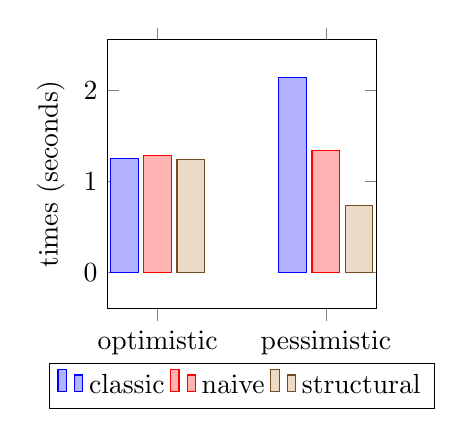
\begin{tikzpicture}
\begin{axis}[
    ybar, ymax = 2, ymin = 0.15,
    enlargelimits=0.3,
    width=5cm, height=5cm,
    legend style={at={(0.5,-0.2)},
      anchor=north,legend columns=-1},
    ylabel={times (seconds)},
    symbolic x coords={optimistic, pessimistic},
    xtick=data
    ]
\addplot coordinates {(optimistic,1.254) (pessimistic,2.142)};
\addplot coordinates {(optimistic,1.282) (pessimistic,1.337)};
\addplot coordinates {(optimistic,1.236) (pessimistic,0.733)};
\legend{classic,naive,structural}
\end{axis}
\end{tikzpicture}
 \captionof{figure}{revers$^o$ forward evaluation \\ for a list with a length of 90}
  \label{fair:plot-reverso}
\end{minipage}%
\begin{minipage}{.5\textwidth}
  \centering
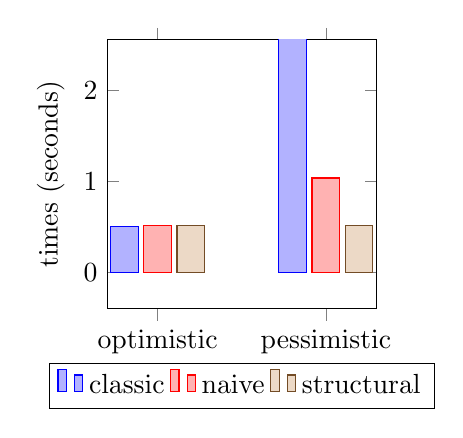
\begin{tikzpicture}
\begin{axis}[
    ybar, ymax = 2, ymin = 0.15,
    enlargelimits=0.3,
    width=5cm, height=5cm,
    legend style={at={(0.5,-0.2)},
      anchor=north,legend columns=-1},
    ylabel={times (seconds)},
    symbolic x coords={optimistic, pessimistic},
    xtick=data
    ]
\addplot coordinates {(optimistic,0.504) (pessimistic,300)};
\addplot coordinates {(optimistic,0.508) (pessimistic,1.035)};
\addplot coordinates {(optimistic,0.513) (pessimistic,0.513)};
\legend{classic,naive,structural}
\end{axis}
\end{tikzpicture}
 \captionof{figure}{sort$^o$ forward evaluation \\ for a list with a length of 5}
\label{fair:plot-sorto}
\end{minipage}
\end{figure*}

\begin{figure*}
\centering
\begin{minipage}{.5\textwidth}
  \centering
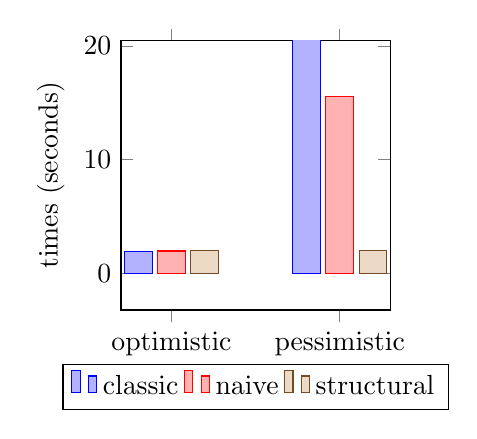
\begin{tikzpicture}
\begin{axis}[
    ybar, ymax = 16, ymin = 1.2,
    enlargelimits=0.3,
    width=5cm, height=5cm,
    legend style={at={(0.5,-0.2)},
      anchor=north,legend columns=-1},
    ylabel={times (seconds)},
    symbolic x coords={optimistic, pessimistic},
    xtick=data
    ]
\addplot coordinates {(optimistic,1.909) (pessimistic,300)};
\addplot coordinates {(optimistic,1.945) (pessimistic,15.516)};
\addplot coordinates {(optimistic,1.980) (pessimistic,1.978)};
\legend{classic,naive,structural}
\end{axis}
\end{tikzpicture}
 \captionof{figure}{``The Tower of Hanoi'' \\ solver evaluation}
\label{fair:plot-hanoi}
\end{minipage}%
\begin{minipage}{.5\textwidth}
  \centering
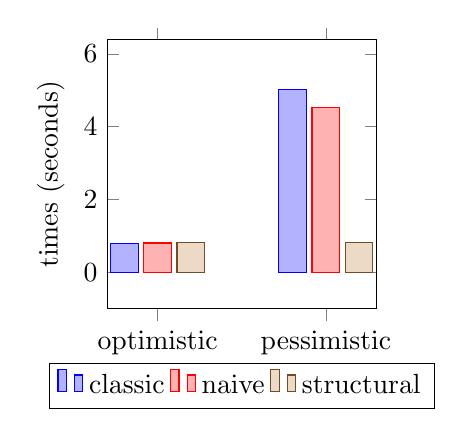
\begin{tikzpicture}
\begin{axis}[
    ybar, ymax = 5, ymin = 0.375,
    enlargelimits=0.3,
    width=5cm, height=5cm,
    legend style={at={(0.5,-0.2)},
      anchor=north,legend columns=-1},
    ylabel={times (seconds)},
    symbolic x coords={optimistic, pessimistic},
    xtick=data
    ]
\addplot coordinates {(optimistic,0.783) (pessimistic,5.019)};
\addplot coordinates {(optimistic,0.801) (pessimistic,4.522)};
\addplot coordinates {(optimistic,0.812) (pessimistic,0.817)};
\legend{classic,naive,structural}
\end{axis}
\end{tikzpicture}
 \captionof{figure}{``Bridge and torch problem'' \\ solver evaluation}
\label{fair:plot-bridge}
\end{minipage}
\end{figure*}

Now we will discuss evaluation. Целью эвалюации является выявления влияния порядка конъюнктов на эффективность трех различных семантик.

Первая семантика с предикатом $pred_{\mbox{\lstinline{true}}}$ близка к классическим реализациям \mk. В дальнейшем будем называть её {\bf left-biased}.

Вторая семантика с предикатом $pred_N$ соответсвует равномерному вычислению всех конъюнктов. Эту семантику будем назвать {\bf naive}.

Третья семантика с предикатом $pred_{\leq_{sr}}$ вычисляет структурно-рекурсивные конъюнкты, пока убывают структурно-рекурсивные аргументы. Её будем называть {\bf structural}.

For evaluation we've chosen two simple programs (list reversing and list sorting) and three more complicated (the ``Hanoi Towers''\footnote{\url{https://en.wikipedia.org/wiki/Tower_of_Hanoi}} solver, the
``Bridge and torch problem''\footnote{\url{https://en.wikipedia.org/wiki/Bridge_and_torch_problem}} solver and ``Water pouring puzzle''\footnote{\url{https://en.wikipedia.org/wiki/Water_pouring_puzzle}} solver).
% Для каждой программы мы сделали две версии. Оптимистичная версия --- это программа, в которой мы вручную подобрали оптимальный порядок конъюнктов и пессиместичная версия --- программа с неоптимальным порядком конъюнктов. В последующих диаграммах и таблице указаны средние значения 10 запусков тестов. Также для наивной равномерной конъюнкции мы подобрали количество разверток вручную. Для равномерной конъюнкции, основанной на структурной рекурсии, N было фиксировано и равно 100.
Each program was written in two versions: ``optimistic'' (with the order of important conjuncts set to provide the best performance) and ``pessimistic'' (with the order of important
conjuncts set to provide the worst performance). Also we evaluated list reversing and list sorting in both directions. In the case of the list reversing, queries \lstinline{(revers$^o$ [1;2;3] q)} and \lstinline{(revers$^o$ q [1;2;3])}\! will give the same answer \lstinline{q = [3;2;1]} but the ``optimistic'' order of conjuncts is different for them. In the case of list sorting, queries \lstinline{(sort$^o$ [1;2;3] q)} and \lstinline{(sort$^o$ q [1;2;3])} will give different answers. The first one gives sorted list \lstinline{q = [1;2;3]}, the second one gives all permutations of list \lstinline{[1;2;3]}\!\!. 

All benchmarks were run ten times, and the average time was taken. For the naive  semantics we cherry-picked the best value of unfolding bound manually. Structural arguments for each relations were detected automatically.

% На изображениях 12-15 представлены результаты апробации в виде столбцовых диаграмм. В оптимистичном случае результаты схожи для всех семантик. В пессиместичном случае время работы напрпавленной конъюнкции резко возрастает, время работы наивной равномерной конъюнкции также ворзрастает, но не так сильно. Равномерная конъюнкция, основанная на структурной рекурсии, демострирует схожую эффективность в сравнении с оптимистичным случаем.
Fig.~\ref{fair:plot-reverso}-\ref{fair:plot-bridge} show the results of evaluation in the form of bar charts. In the optimistic case, the results are similar for all semantics.
In the pessimistic case the evaluation time of the directed conjunction rapidly increases, the evaluation time of the naive fair conjunction also increases, but not so much.
The fair semantics based on structural recursion demonstrates a similar efficiency as in the optimistic case.

\begin{figure*} %[h!]
  \small
  \centering
  \begin{tabular}{ c | c | c | c | c | c | c | c }
    \multirow{2}{*}{relation} & \multirow{2}{*}{size} & 
    \multicolumn{2}{c}{left-biased semantics} &
    \multicolumn{2}{c}{naive semantics} &
    \multicolumn{2}{c}{structural semantics} \\
    \cline{3-8}
    & & optimistic & pessimistic & optimistic & pessimistic & optimistic & pessimistic  \\ 
    \hline
    \multirow{3}{*}{\begin{tabular}{c} forward \\ revers$^o$ \end{tabular}}
                 & 30   & 0.527 & 0.587  & 0.532 & 0.595   & 0.539 & 0.532 \\
                 & 60   & 0.639 & 0.947  & 0.643 & 0.790   & 0.657 & 0.577 \\
                 & 90   & 1.254 & 2.142  & 1.282 & 1.337   & 1.236 & 0.733 \\
    \hline
    \multirow{3}{*}{\begin{tabular}{c} backward \\ revers$^o$ \end{tabular}}
                 & 30   & 0.531 & 0.579  & 0.547 & 0.570  & 0.553 & 0.563 \\
                 & 60   & 0.655 & 0.875  & 0.667 & 0.812  & 0.668 & 0.681 \\
                 & 90   & 1.316 & 1.813  & 1.327 & 1.503  & 1.360 & 1.359 \\
    \hline
    \multirow{5}{*}{\begin{tabular}{c} forward \\ sort$^o$ \end{tabular}}
                 & 3    & 0.467 & 0.503  & 0.474 & 0.481  & 0.472 & 0.479 \\
                 & 4    & 0.484 & 4.679  & 0.485 & 0.493  & 0.490 & 0.488 \\
                 & 5    & 0.504 & $>$300 & 0.508 & 1.035  & 0.513 & 0.513 \\
                 & 6    & 0.526 & $>$300 & 0.237 & 14.369 & 0.544 & 0.547 \\
                 & 30   & 1.915 & $>$300 & 1.936 & $>$300 & 1.983 & 1.987 \\
    \hline
    \multirow{4}{*}{\begin{tabular}{c} backward \\ sort$^o$ \end{tabular}}
                 & 3    & 0.518 &  0.519 & 0.518 & 0.521  & 0.520 & 0.521 \\
                 & 4    & 0.533 &  0.856 & 0.534 & 0.540  & 0.534 & 0.537 \\
                 & 5    & 0.680 & 93.914 & 0.713 & 1.528  & 0.718 & 0.714 \\
                 & 6    & 2.931 & $>$300 & 2.947 & 59.647 & 2.938 & 2.936 \\
    \hline
    hanoi$^o$    & -    & 1.909 & $>$300 & 1.945 & 15.516 & 1.980 & 1.978 \\
    \hline
    bridge$^o$   & -    & 0.783 & 5.019  & 0.801 & 4.522  & 0.812 & 0.817 \\
    \hline
    water$^o$    & -    & 3.513 & $>$300 & 3.518 & $>$300 & 3.538 & 3.771

  \end{tabular}
  \caption{The results of evaluation: running times of benchmarks in seconds}
  \label{fair:evaluation-table}
\end{figure*}

% Более подробно результаты представлены на изображении 16. Можно заметить, что время работы программы sorto в пессиместичном случае очень быстро растет с увеличением длины списка для направленной конъюнкции и наивной равномерной. В случае с равномерной конъюнкцией, основанной на структурной рекурсии, пессиместичный случай растет сопостовимо с оптимистичным.
The results are presented in more detail in Fig.~\ref{fair:evaluation-table}. ``Hanoi Towers'' solver has name \lstinline{hanoi$^o$}, ``Bridge and torch problem'' solver has name \lstinline{bridge$^o$} and ``Water pouring puzzle'' solver has name \lstinline{water$^o$}. We can conclude that forward and backward \lstinline{sort$^o$} runtime in the pessimistic case increases very rapidly with increasing the list length for left-biased and naive fair semantics. In the case of the fair semantics based on structural recursion the running time in pessimistic case increases on a par with that in the optimistic one. Also the solver \lstinline{water$^o$} very slow in the pessimistic case for left-biased and naive fair. However, fair conjunction based on structural recursion pessimistic case is no different from an optimistic case.


% Подводя итог, равномерная конъюнкция, основанная на структурной рекурсии сопоставима по эффективности с направленной конъюнкцией. Более того, это конъюнкция слабо зависит от порядка конъюнктов.
To summarize, the fair semantics based on structural recursion does not introduce any essential overhead in comparison with left-biased semantics in an optimistic case. At the same time it
weakly depends on the order of the conjuncts, and thus demonstrates much better performance in the pessimistic case.

\section{Conclusion}
\label{conclusion}

We presented an approach for converting typed functional programs into relations. Relational conversion 
in many cases allows us to avoid tedious recoding of functional specifications into relational form and to 
concentrate on writing relational specifications only when their reconstruction from functions is impossible or 
undesirable. Our implementation works for the subset of OCaml; we evaluated it for a number of interesting 
examples and acquired some new relational solutions.

There is a number of directions for future research. First, a performance evaluation is desirable~--- at
present time we do not know, what slowdown factor is. Another problem is a development of an approach to
prove complete correctness (or refute this claim).


\bibliographystyle{splncs04}
\bibliography{references}
\end{document}
